\documentclass[twocolumn, 8pt]{extarticle}
\usepackage{amsmath}
\usepackage{graphicx}
\usepackage{multicol}
\usepackage{float}
\usepackage[paper=a4paper, margin=1cm]{geometry}

\graphicspath{ {./images/} }
\pagenumbering{gobble}
\setlength{\parindent}{0pt}
\setlength{\columnsep}{2cm}
\setlength{\columnseprule}{0.4pt}

\begin{document}

\section*{\underline{Arrays}}
\( \vec{E}_{dipolo} = j \eta \frac{ e^{-jkr} }{ 2 \pi r } I \frac{ \cos\left(\frac{\pi}{2} \cos(\theta)\right) }{\sin{\theta}} \hat{\theta} ,\ \eta = 120\pi \)

\vspace{0.5cm}
\( Z_{dip}^{\lambda / 2} = 73 + j42 \  \Omega \)

\vspace{0.5cm}
\( \left|FA(\psi)\right| = \left|\frac{ \sin(N \frac{\psi}{2}) }{ \sin(\frac{\psi}{2}) } \right|\)

\vspace{0.5cm}
\( D_{max} = \frac{ S_{max} }{ P_{rad} / 4 \pi r^2}  = \frac{120}{R^{tot}_{in-dip}}N^2_{dip} \)

\vspace{0.5cm}
\( D_{boradside} \simeq  2N \dfrac{d}{\lambda}\)

\vspace{0.5cm}
\( D_{endfire} \simeq  4N \dfrac{d}{\lambda}\)

\vspace{0.5cm}
\( \text{Margen visible: } [-kd + \alpha,\ kd + \alpha] \)

\vspace{0.5cm}
\(\left \{
\begin{array}{l}
    k_x = k \sin(\theta) \cos(\varphi) \\
    k_y = k \sin(\theta) \sin(\varphi) \\
    k_z = k \cos(\theta)
\end{array}
\right .
\)

\vspace{0.5cm}
\( \text{Distancia entre nulos: } \frac{ 2\pi }{ N }, \frac{ 4\pi }{ N } , ... \ , 2\pi \)

\vspace{0.5cm}
\( NLPS = 20 \log_{10} \left(\frac{ N }{\left|FA\left(\frac{ 3\pi }{ 2N }\right)\right|} \right) = 20 \log_{10} \left(N \sin\left( \frac{ 3\pi }{ 2N }\right)\right) dB \)

\vspace{0.5cm}
\( RDA = 20 \log_{10} \left( \frac{ \left|FA(0)\right| }{ \left|FA(-2kd))\right| } \right) dB \)

\vspace{0.5cm}
\( \text{Acoplamientos mutuos: } \left \{
\begin{array}{l}
    V_i = Z_{i1}I_1 + Z_{i2}I_2 + \dots + Z_{ij}I_j \\ \\
    Z_i = \frac{V_i}{I_i} = Z_{i1} \frac{I_1}{I_i} + Z_{i2} \frac{I_2}{I_i} + \dots + Z_{ij} \frac{I_j}{I_i}
\end{array}
\right .
\)

\vspace{0.5cm}
\section*{\underline{Bocinas}}

\( \vec{E}_{apertura} = E_0 \cos \left( \frac{\pi}{a_g}x \right) \hat{y} \)

\vspace{0.5cm}
\( s = \frac{ b^2 }{ 8\lambda L_E}, \ s_{opt} = \frac{1}{4} \)

\vspace{0.5cm}
\( t = \frac{ a^2 }{ 8\lambda L_H}, \ t_{opt} = \frac{3}{8} \)

\vspace{0.5cm}
Error de fase: \( \left \{
\begin{array}{l}
    2\pi s \\
    2\pi t
\end{array}
\right . \)

\vspace{0.5cm}
\( b_{opt} = \sqrt{ 2\lambda L_E } \)

\vspace{0.5cm}
\( a_{opt} = \sqrt{ 3\lambda L_H } \)

\vspace{0.5cm}
\( D_{pir} = \frac{ 4\pi }{ \lambda^2 } A_{eff} = \frac{ 4\pi }{ \lambda^2 } A_{geom} \, \eta_{il} = \frac{ 4\pi }{ \lambda^2 } a \, b \, \eta_{il_x} \eta_{il_y} \)

\vspace{0.5cm}
\( \eta^{opt}_{il ,\, pir} \simeq 0.5188 \)

\vspace{0.5cm}
\( \eta^{opt}_{il ,\, H} =  \eta^{opt}_{il ,\, E} \simeq 0.6485 \)

\newpage
\section*{\underline{Reflectores}}

\( R = f + (f - R\cos(\alpha)) \Rightarrow R = \frac{2f}{1 + cos(\alpha)} = \frac{f}{\cos^2\left(\frac{\alpha}{2}\right)}\)

\vspace{0.5cm}
\( \rho = R \sin(\alpha) = 2f \tan\left(\frac{\alpha}{2}\right) \)

\vspace{0.5cm}
\( \tau_c = 40\log_{10}\left(\cos\left(\frac{\beta}{2}\right)\right) dB \)

\vspace{0.5cm}
\( \frac{f}{D} = \frac{1}{4\tan\left(\frac{\beta}{2}\right)} \)

\newpage

\begin{multicols}{2}
    \begin{figure}[H]
        \centering
        \textbf{Broadside}
        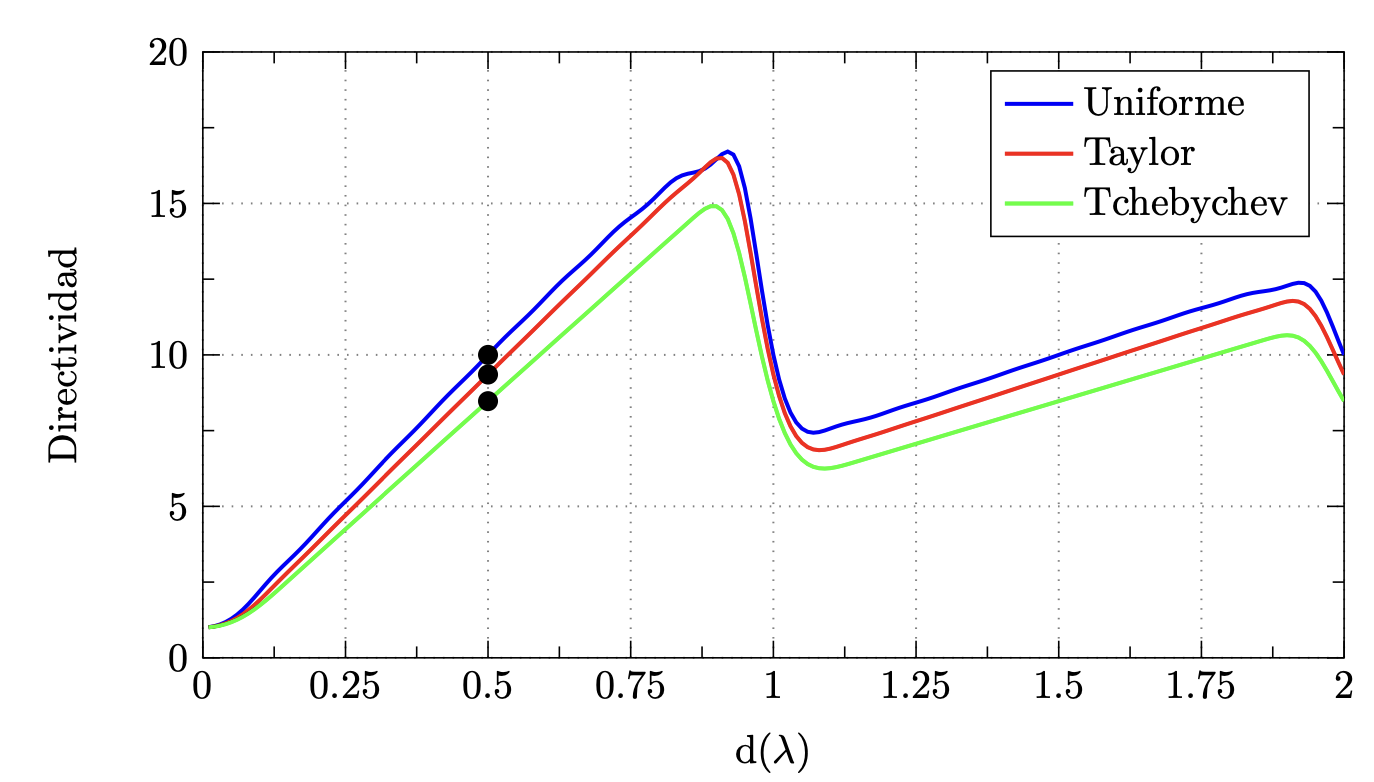
\includegraphics[width=\columnwidth]{directividad_broadside.png}
    \end{figure}

    \begin{figure}[H]
        \centering
        \textbf{Endfire}
        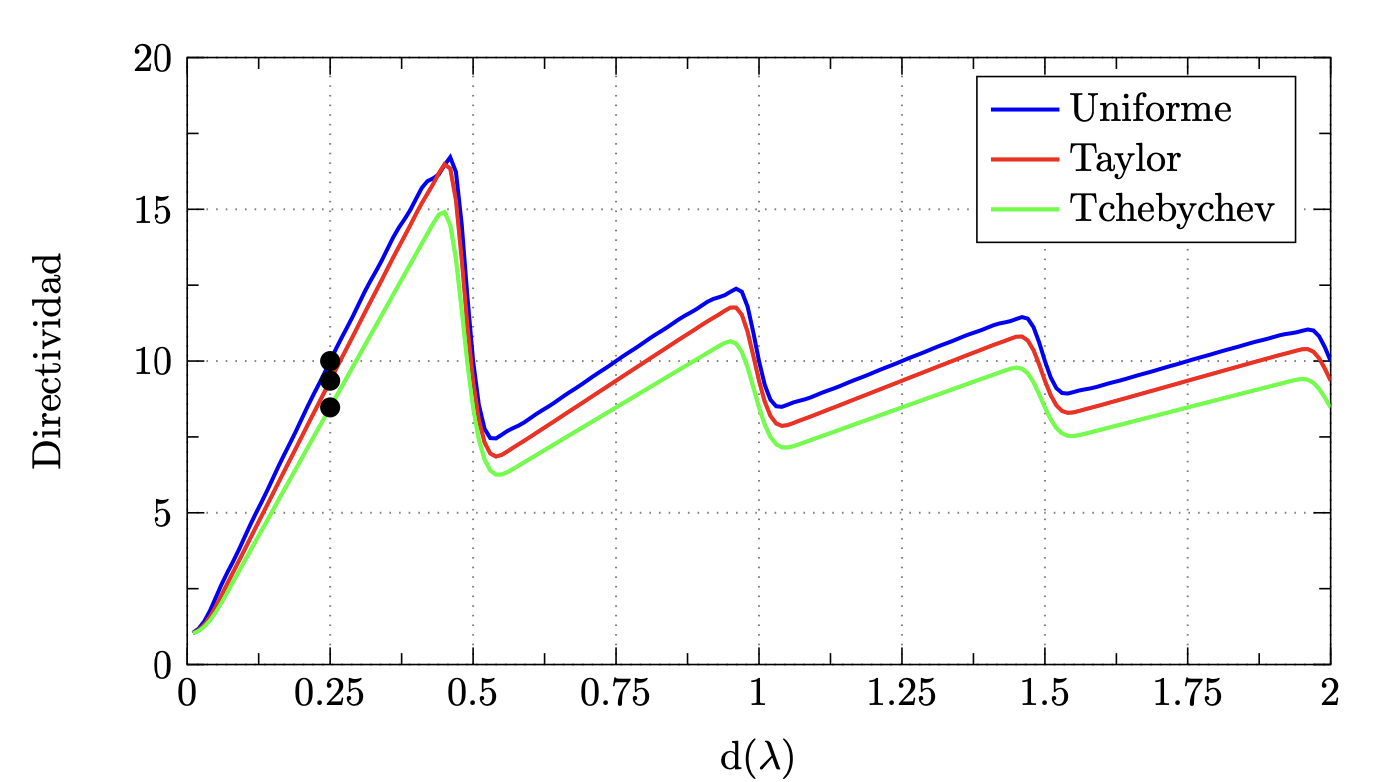
\includegraphics[width=\columnwidth]{directividad_endfire.png}
    \end{figure}
\end{multicols}

\begin{figure}[H]
    \centering
    \textbf{Bocinas}
    \centering
    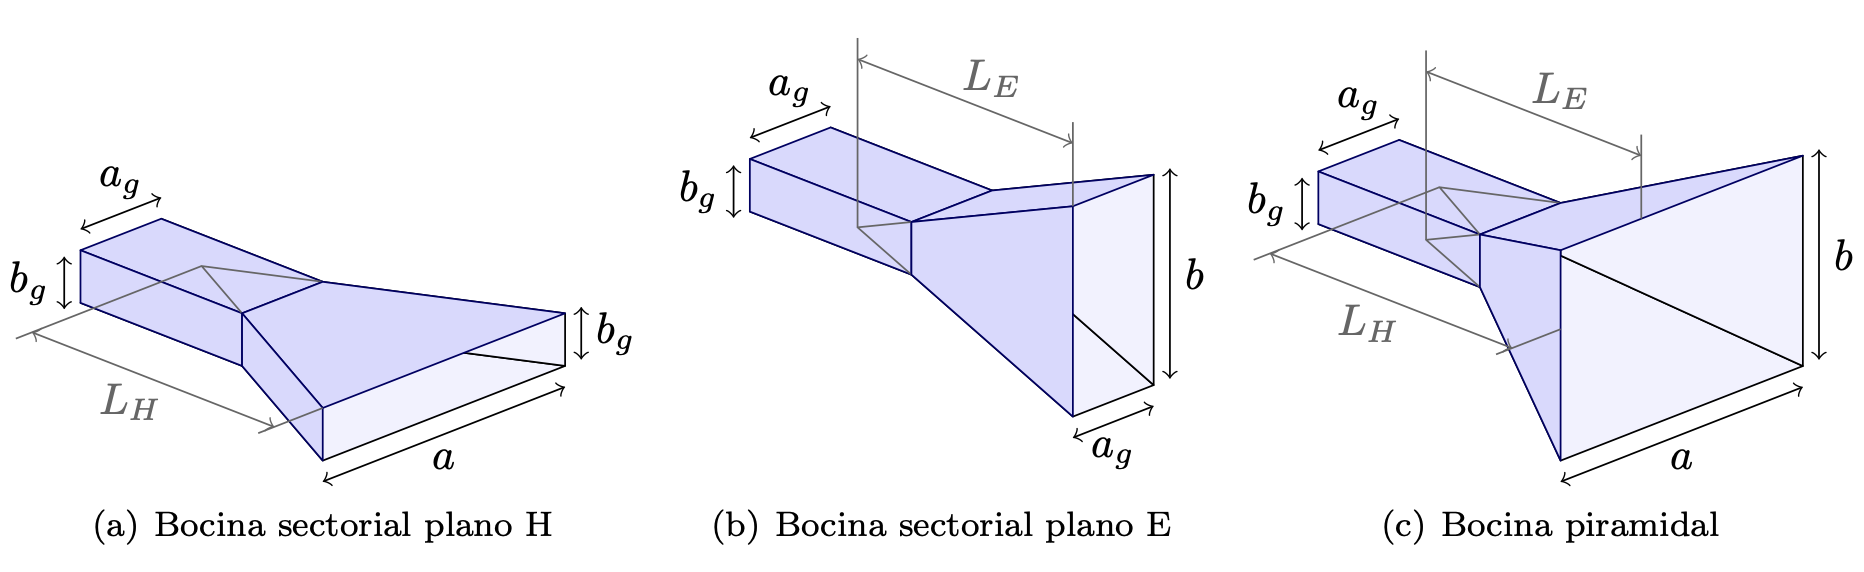
\includegraphics[width=\columnwidth]{bocinas.png}
\end{figure}

\begin{multicols}{2}
    \begin{figure}[H]
        \centering
        \textbf{Plano E}
        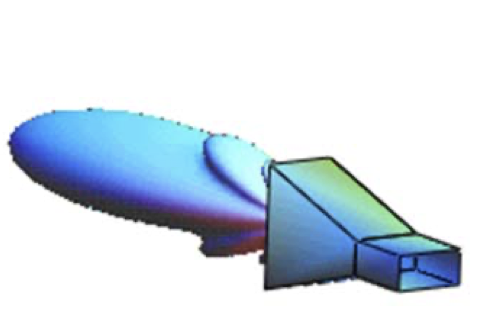
\includegraphics[width=\columnwidth]{bocina_e.png}
    \end{figure}

    \begin{figure}[H]
        \centering
        \textbf{Plano H}
        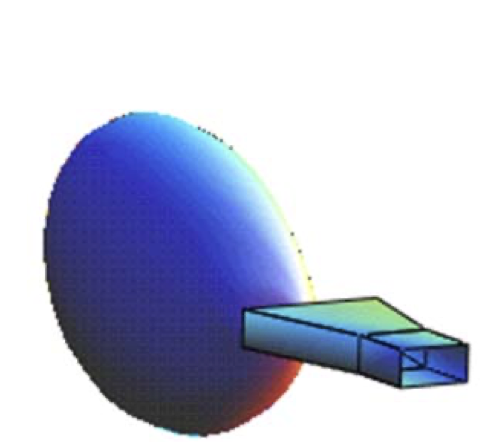
\includegraphics[width=\columnwidth]{bocina_h.png}
    \end{figure}
\end{multicols}

\begin{figure}[H]
    \centering
    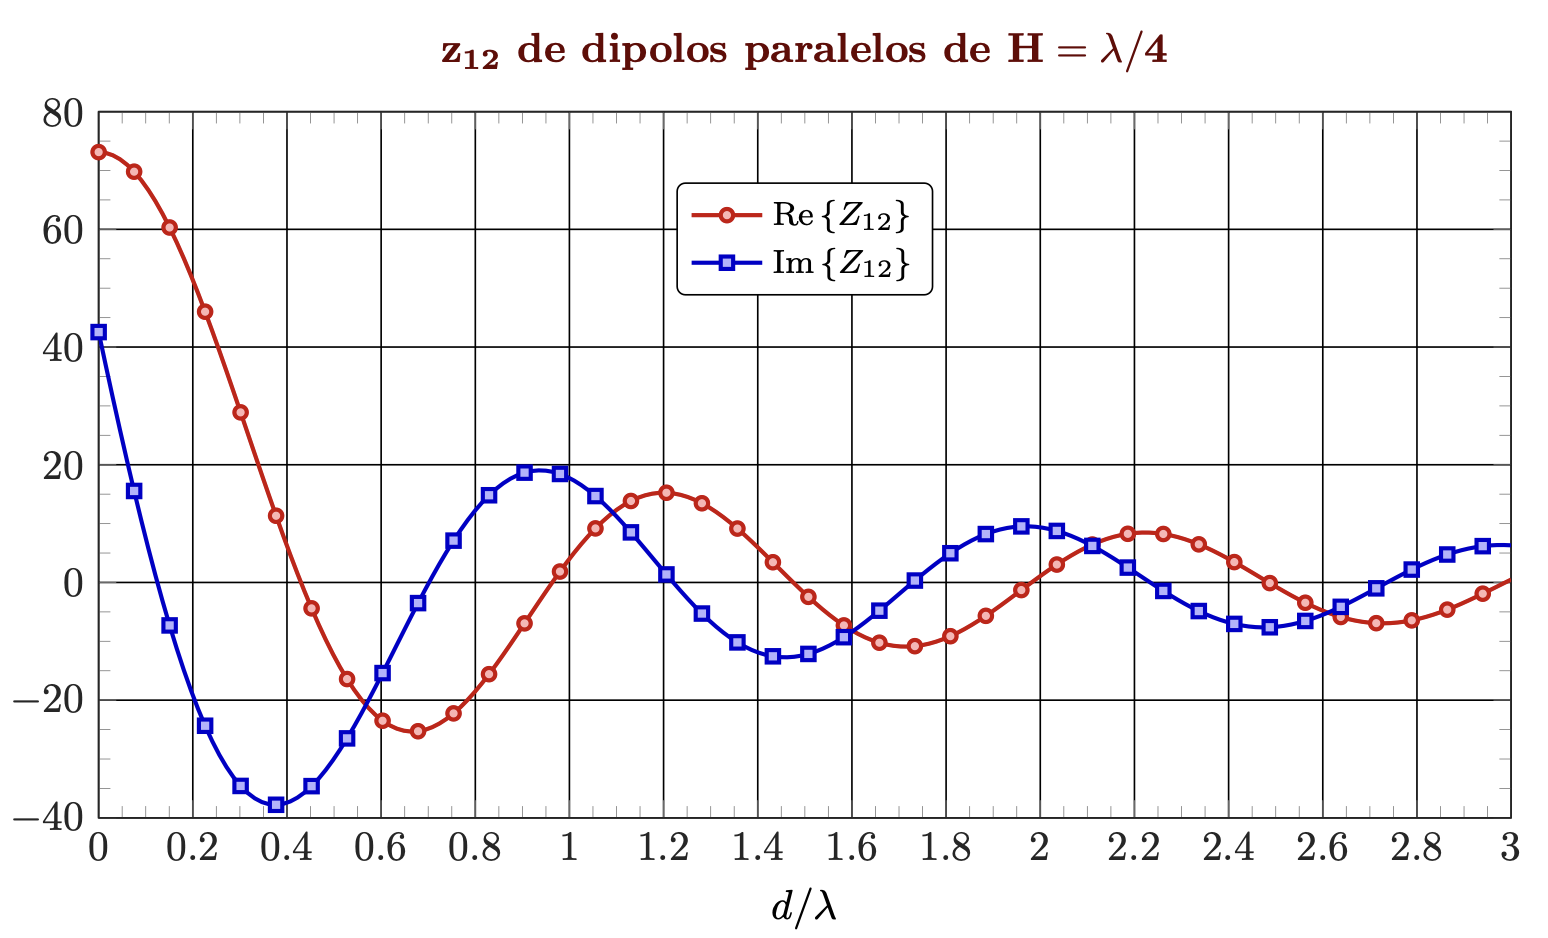
\includegraphics[width=\columnwidth]{z_dipolos.png}
\end{figure}

\begin{figure}[H]
    \centering
    \textbf{Factor de array para N = 10}
    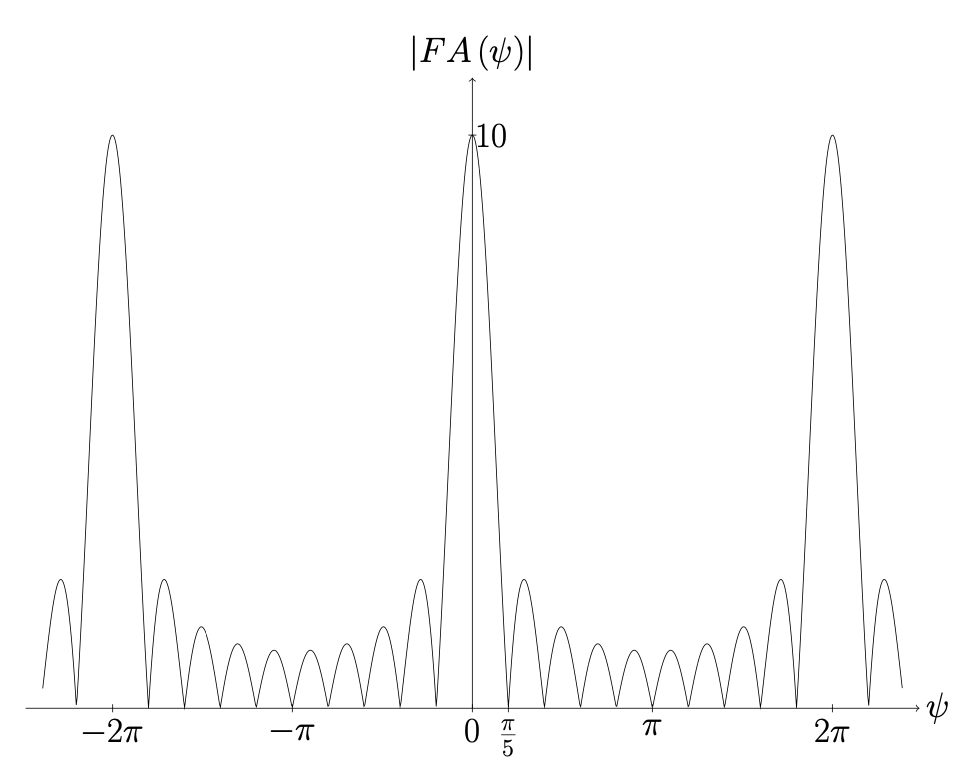
\includegraphics[width=\columnwidth]{fa.png}
\end{figure}

\newpage

\begin{figure}[H]
    \centering
    \textbf{Reflector Parabolico}
    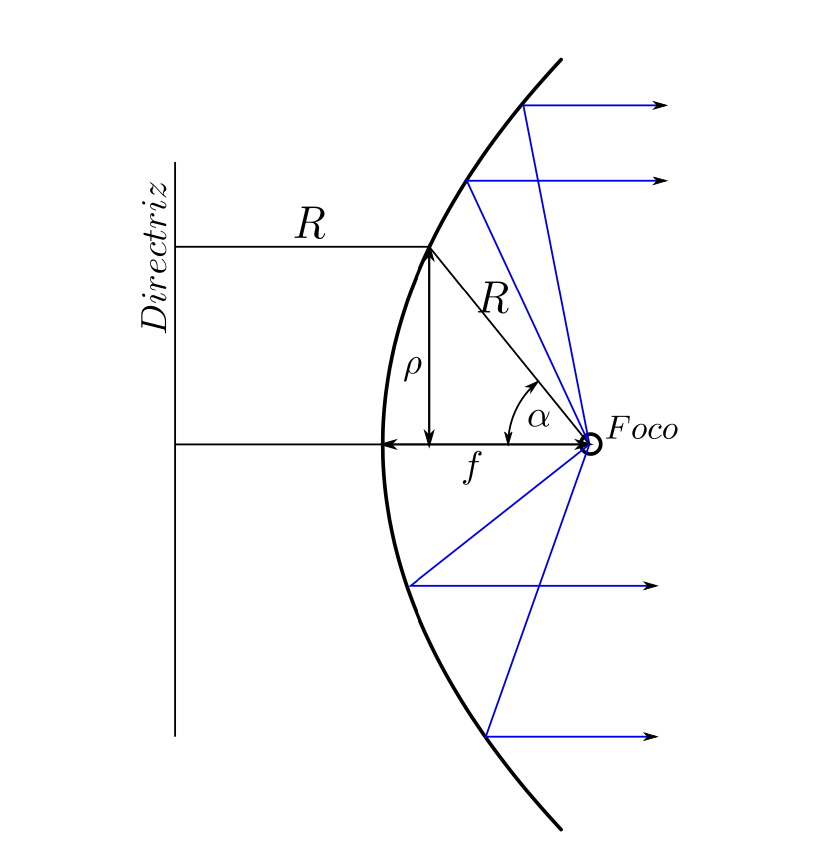
\includegraphics[width=\columnwidth]{reflector.png}
\end{figure}

\begin{multicols}{2}
    \begin{figure}[H]
        \centering
        \textbf{Reflector plano E}
        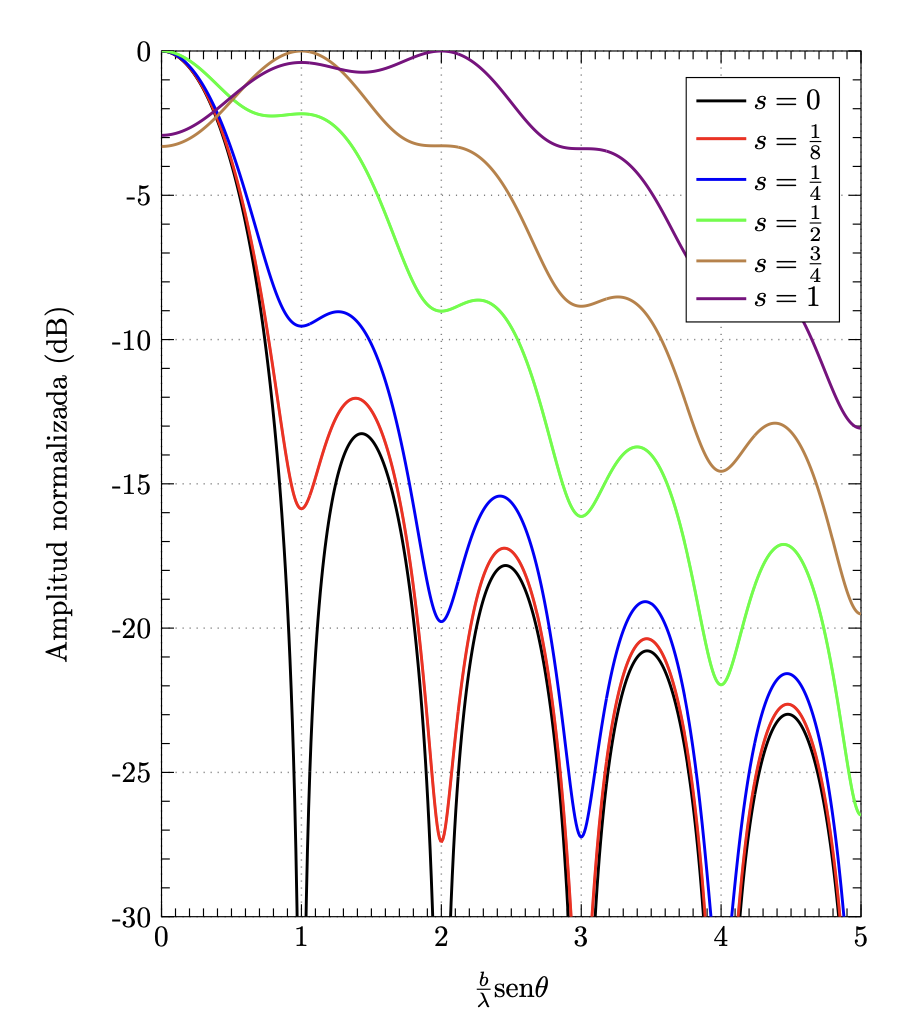
\includegraphics[width=\columnwidth]{reflector_plano_e.png}
    \end{figure}

    \begin{figure}[H]
        \centering
        \textbf{Reflector plano H}
        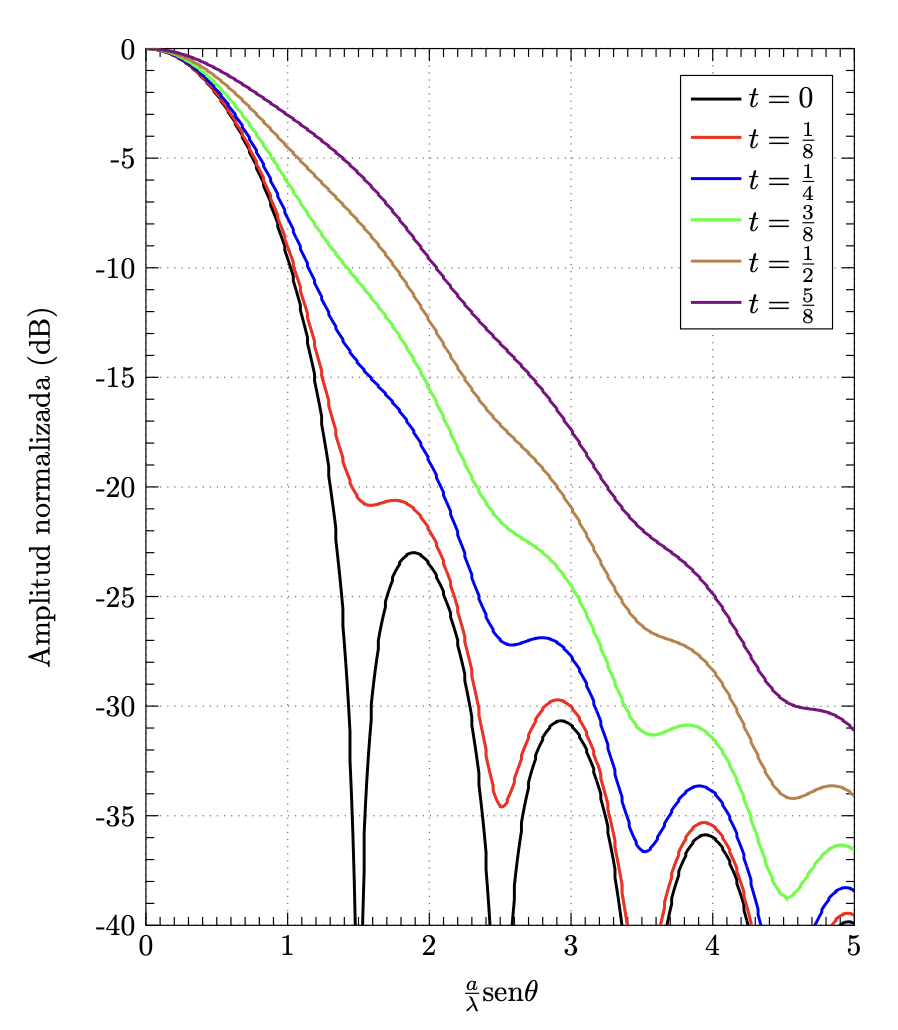
\includegraphics[width=\columnwidth]{reflector_plano_h.png}
    \end{figure}
\end{multicols}

\begin{figure}[H]
    \centering
    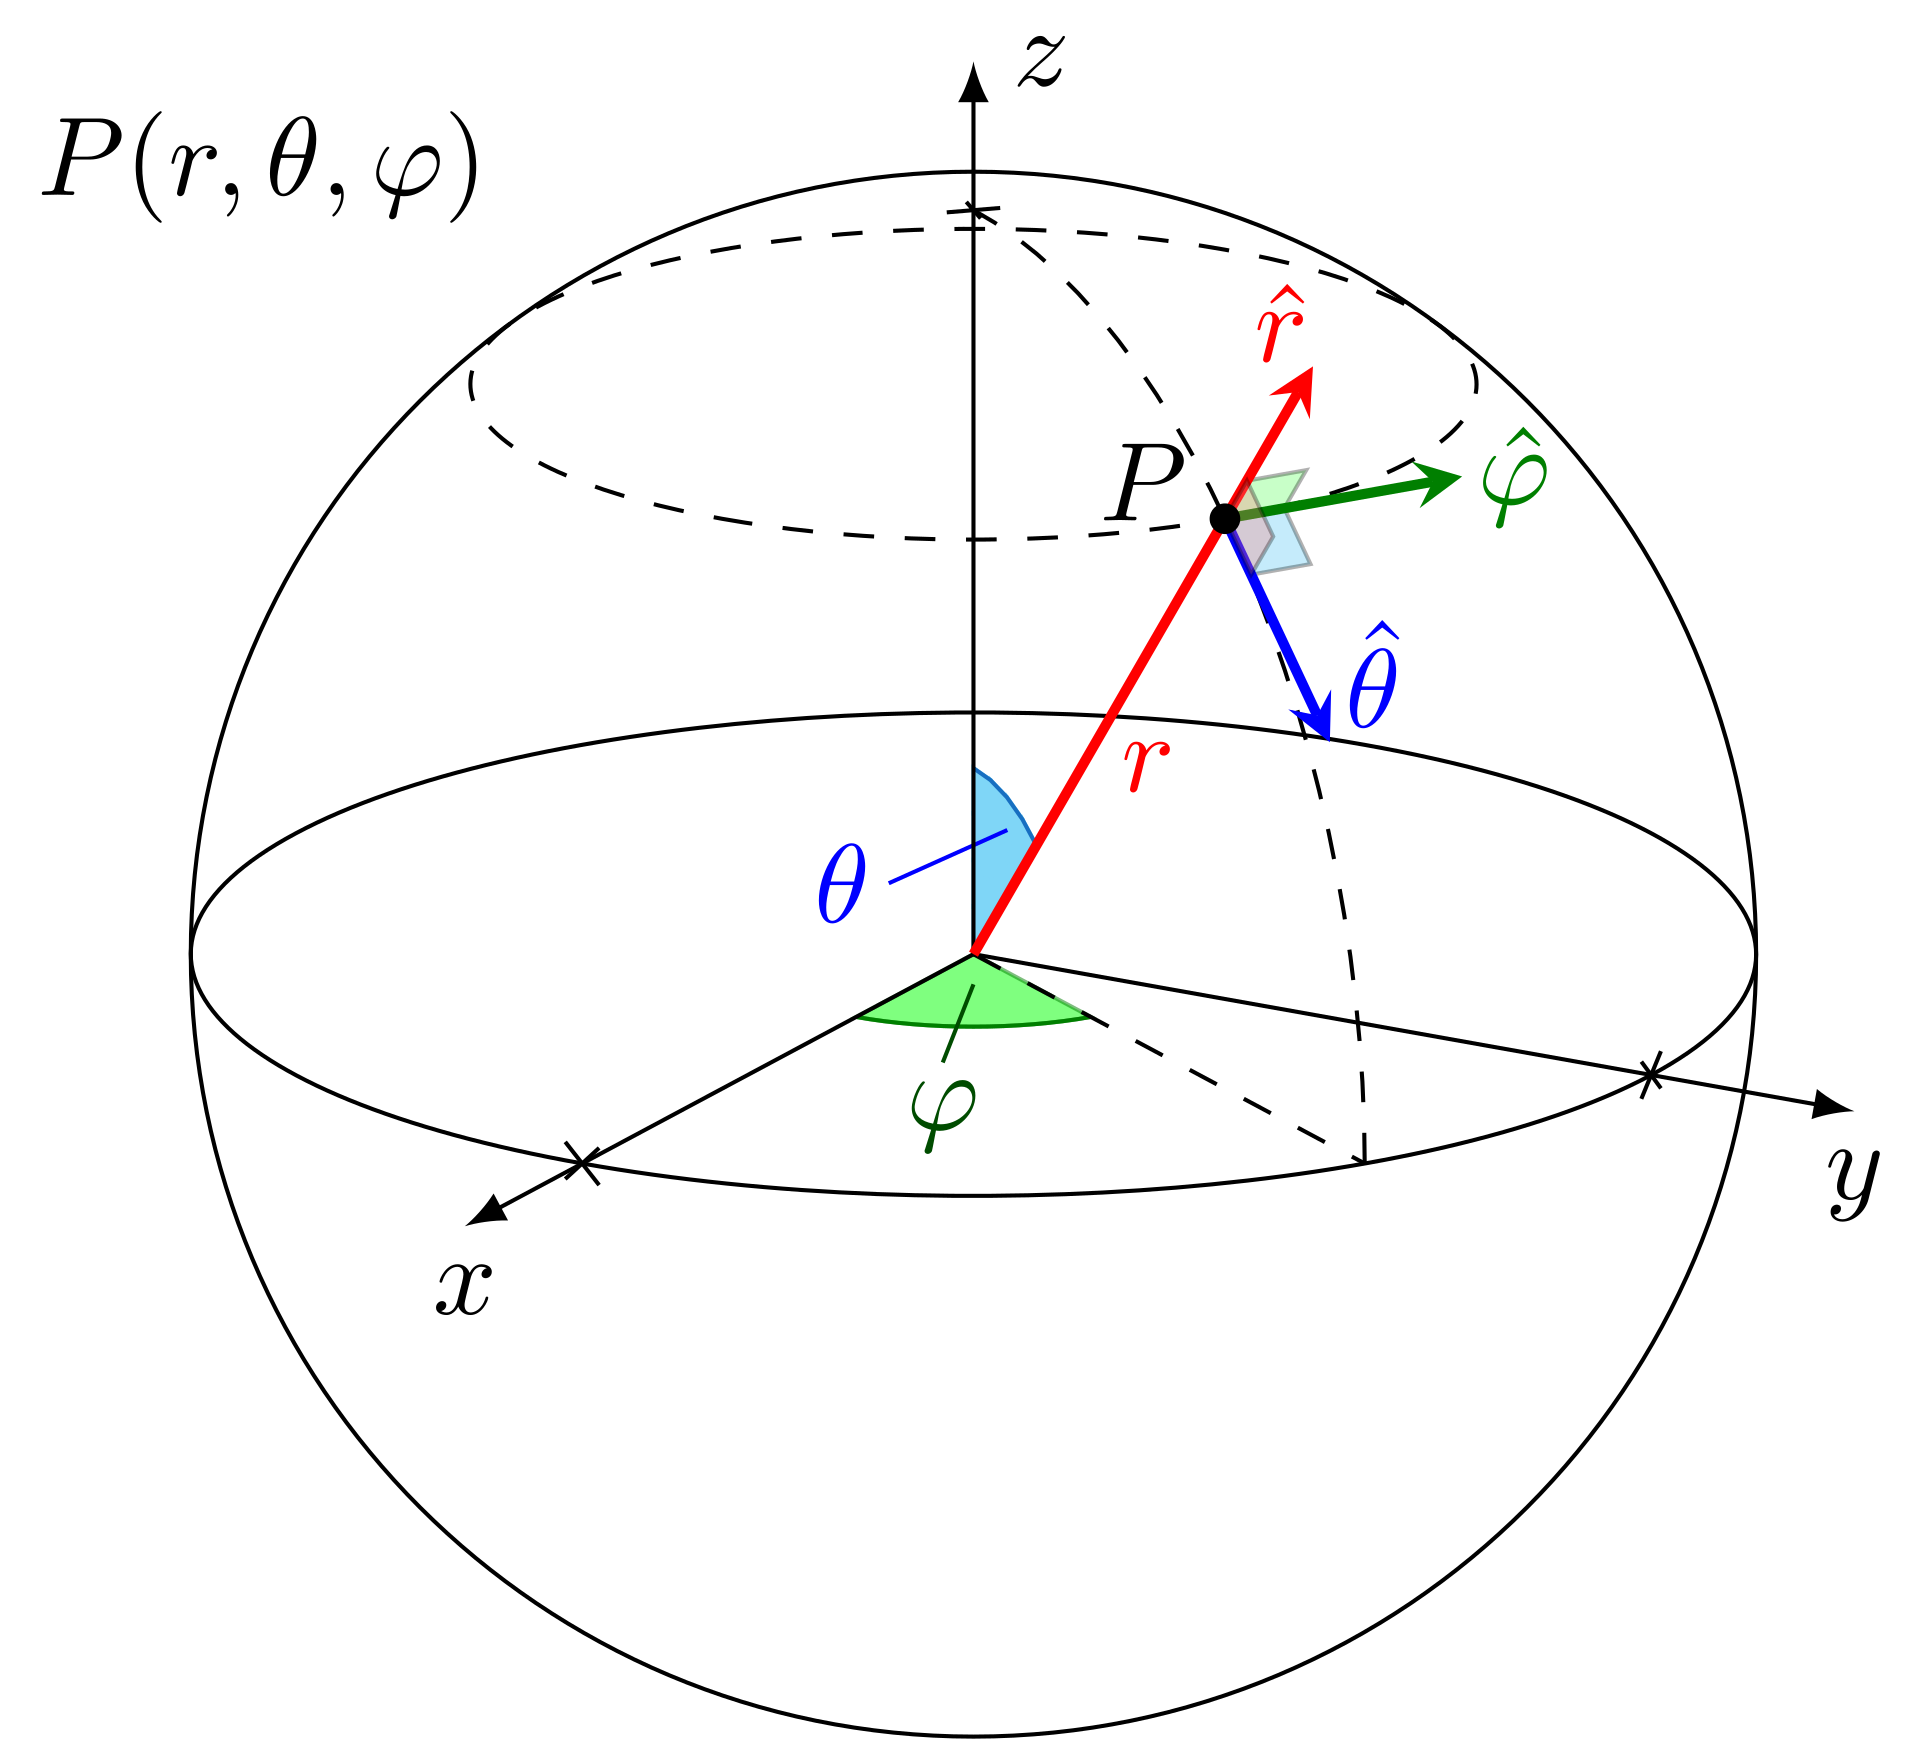
\includegraphics[width=\columnwidth]{esfericas.png}
    \vspace{0.1cm}


    \(x = r \sin(\theta) \cos(\varphi)\)\\
    \(y = r \sin(\theta) \sin(\varphi)\)\\
    \(z = r \cos(\theta)\)
\end{figure}

\end{document}